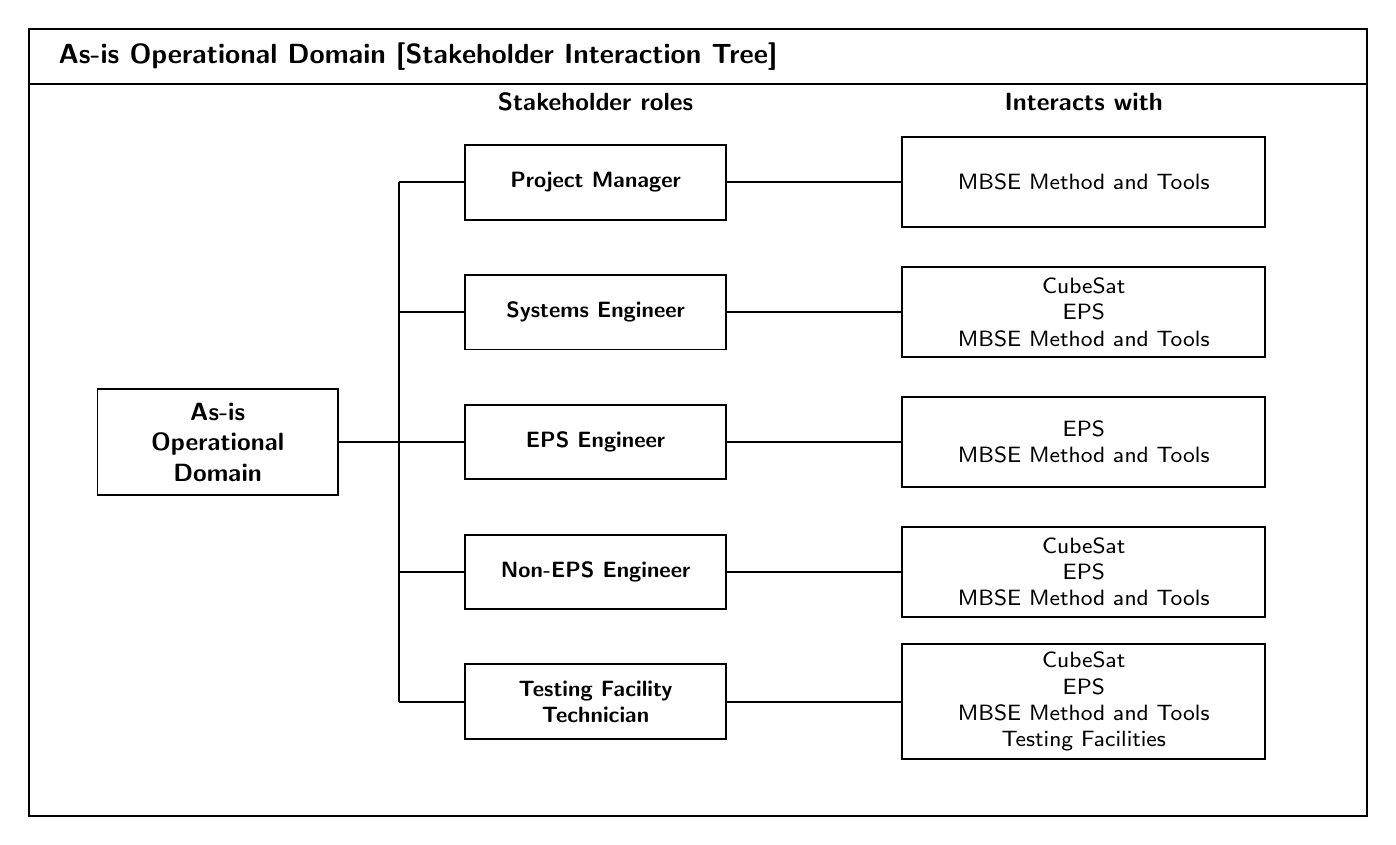
\begin{tikzpicture}[
  font=\sffamily,
  line width=0.7pt,
  domainblock/.style={
    draw,
    align=center,
    text width=2.7cm,
    minimum height=1.25cm,
    inner sep=5pt,
    fill=white,
    font=\sffamily\small\bfseries
  },
  role/.style={
    draw,
    align=center,
    text width=3.1cm,
    minimum height=0.95cm,
    inner sep=3pt,
    fill=white,
    font=\sffamily\footnotesize\bfseries
  },
  targets/.style={
    draw,
    align=center,
    text width=4.4cm,
    minimum height=1.15cm,
    inner sep=3pt,
    fill=white,
    font=\sffamily\footnotesize
  }
]
  \draw (0,0) rectangle (17,10);
  \node[anchor=west,font=\sffamily\bfseries] at (0.25,9.65)
    {As-is Operational Domain [Stakeholder Interaction Tree]};
  \draw (0,9.3) -- (17,9.3);

  \node[anchor=south,font=\sffamily\small\bfseries] at (7.2,8.83) {Stakeholder roles};
  \node[anchor=south,font=\sffamily\small\bfseries] at (13.4,8.83) {Interacts with};
  \node[domainblock] (domain) at (2.4,4.75) {As-is\\Operational Domain};

  \node[role] (manager) at (7.2,8.05) {Project Manager};
  \node[role] (systems) at (7.2,6.4) {Systems Engineer};
  \node[role] (epsEngineer) at (7.2,4.75) {EPS Engineer};
  \node[role] (nonEps) at (7.2,3.1) {Non-EPS Engineer};
  \node[role] (technician) at (7.2,1.45) {Testing Facility\\Technician};

  \node[targets] (managerTargets) at (13.4,8.05) {MBSE Method and Tools};
  \node[targets] (systemsTargets) at (13.4,6.4)
    {CubeSat\\EPS\\MBSE Method and Tools};
  \node[targets] (epsTargets) at (13.4,4.75)
    {EPS\\MBSE Method and Tools};
  \node[targets] (nonEpsTargets) at (13.4,3.1)
    {CubeSat\\EPS\\MBSE Method and Tools};
  \node[targets] (technicianTargets) at (13.4,1.45)
    {CubeSat\\EPS\\MBSE Method and Tools\\Testing Facilities};

  \draw (domain.east) -- (4.7,4.75);
  \draw (4.7,1.45) -- (4.7,8.05);
  \foreach \person/\resource/\y in {
    manager/managerTargets/8.05,
    systems/systemsTargets/6.4,
    epsEngineer/epsTargets/4.75,
    nonEps/nonEpsTargets/3.1,
    technician/technicianTargets/1.45
  } {
    \draw (4.7,\y) -- (\person.west);
    \draw (\person.east) -- (\resource.west);
  }

\end{tikzpicture}
